\chapter{Virtualization and Cloud Computing}
\label{chapter:cloudcomputing}

%General about the shift that has been happening towards virtualized and software applications

Virtualization is technology that lets you create useful IT services using resources that are traditionally bound to hardware. Virtualization allows hardware operators to use the physical machine's full capacity by distributing the computing power to multiple users or environments. \cite{RedHat} In the context of telco, virtualization the main objective is to replace the costly dedicated hardware implementing several centralized control plane functions and other services with distributed solutions that may be allocated on-demand over a pool of dependable, dynamically contracted computing and networking resources that are easy to manage. \cite{Bosch2011} Virtualization brings down the expenses arising from acquiring, updating and managing the hardware. 

\section{Cloud computing}

Data centers, with the help of hardware virtualization, offer on-demand availability of computer resources such as computing power or data storage. This pay-per-use offering is described as cloud computing. It has been a vital enabler in the field of Information Technologies allowing the success of cloud applications such Google Docs, Slack, and Dropbox. The ubiquitous and connected computing provided allows higher usage of resources and access from anywhere via internet, thus improving performance, reducing costs, and allowing easy access to hosted applications.

A cloud is a pool of virtualized resources across the internet, that follows pay-per-use model and can be dynamically reconfigured to satisfy the user requests by provisioning virtual machines. Cloud computing is a service model for IT provisioning, often based on virtualization and distributed computing technologies \cite{Lombardi2011}. Cloud is typically a centralized server, such as, Microsoft Azure or Red Hat OpenShift. These cloud platforms provide users with scalable resources, high availability and fast connections. Cloud platforms can be public, such as the before-mentioned ones, or a private cloud serving only selected customers. Private clouds are usually deployed on-premises within a corporate firewall by businesses with requirements for additional control and privacy over the network. \cite{MicrosoftAzure}

Hybrid cloud is a combination of both, made up of on-premises infrastructure, private cloud services, and a public cloud. The hybrid approach brings enterprise with agility to use the best suitable solution for each occasions. \cite{NetApp} Community cloud is a resource pool that consists of an aggregation of several providers, which can be shared by a certain group of users. \cite{Taleb2017}

% Service models? 

\section{Virtualization types}

The traditional server has applications running on the host operating system (OS). The solution limits overhead from extra layers such as hypervisor or virtual machine (VM), but compromises the usage of resource efficiency, security and limits compatibility. Two virtualization technologies, hypervisor-based virtualization and operating system -level virtualization, have been introduced to improve these features. Figure \ref{fig:VirtualizationTypes} describes the stack of these two virtualization types and a traditional physical server.

\begin{figure}[ht]
  \begin{center}
    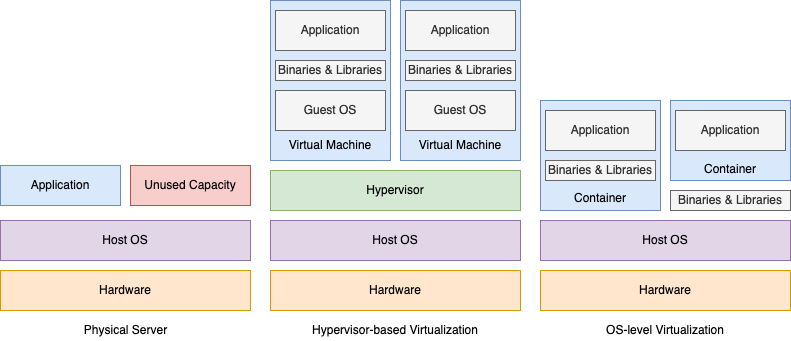
\includegraphics[width=13.5cm]{LaTeX/images/VirtualizationTypes.png}
    \caption{Physical server and two types of virtualization}
    \label{fig:VirtualizationTypes}
  \end{center}
\end{figure}

First of the virtualization technologies, hypervisor-based virtualization adds a hypervisor on top of the host OS and each application instance running is wrapped inside a VM with a dedicated guest OS, binaries, and libraries. This approach is secure and compatible with various host operating systems and processor architectures via hardware emulation. However, the added layers increase the performance overhead significantly. Resources of the server are wasted, especially when multiple VMs are hosted on the same server. In contrast, OS-level virtualization with containers replace the bulky OS with minimal image, such as Alpine. Containers are isolated areas in the host operating system and they do not include an additional guest operating system inside them. Instead, to enable operating system-like functionality, they share parts of the host kernel as well as the host’s libraries and binaries where appropriate. These containers can also include application specific binaries and libraries. \cite{Toimela2017} 

\subsection{Security concerns}

In order to mitigate costs from the application, it is resource-efficient to run multiple instances or different applications in a single server. This applies to companies who own dedicated servers or cloud computing providers with various data center options. These multi-tenant environments may host applications also from untrusted parties. Regardless of the isolation offered by Docker with cgroups and namespaces, the kernel is still shared between the containers. This architectural decision might lead to exposing applications, as it was noticed in 2019 \cite{CVE-2020-14386}\cite{CVE-2019-5736} when attackers could elevate their access to host root. The escaping of container and horizontal traversal via shared kernel creates a security thread of application data integrity.

%You can translate your latex file to rtf with the \texttt{latex2rtf} command in the
%kosh.aalto.fi shell server. Then, the line breaks
%will not be problems for the proofreader of Word.

%Note also that if you have a section or a subsection, you have to have
%at least two of them, or otherwise the section or subsection title is
%unnecessary. Same with the paragraphs: you should not have sections
%with only one paragraph, and single sentence paragraph.

%Aalto library has a comprehensive citation guide ~\cite{bibinstructions}.